\chapter{Object Detection as Regression}
\label{ch:lesson41}

Chapter~\ref{ch:lesson40}'s sliding-window detector classified thousands of fixed-size windows and merged the results with non-maximum suppression (NMS). That works, but it is fundamentally a \emph{classification} approach bolted onto a search --- the network never predicts a box directly, only ``face or not, at this exact window.'' Modern detectors instead treat localization as a \textbf{regression} problem: given an image, directly predict bounding box coordinates. This chapter builds the simplest possible version of that idea, then surveys how real detectors (R-CNN, YOLO, SSD) scale it up.

\section{One object per image: predict a box directly}

The simplest possible regression problem: one circular blob per image, at an unknown location and size (Figure~\ref{fig:l41-1}). Instead of a class label, the network's target is now four numbers --- $(c_x, c_y, w, h)$ indicating the bounding box, normalized to $[0,1]$ by image size.

\begin{figure}[h]
\centering
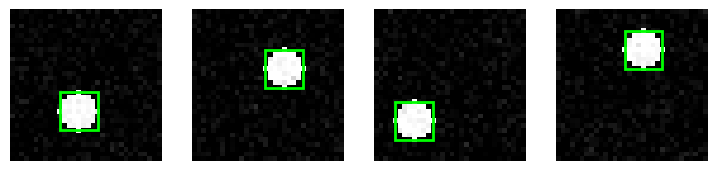
\includegraphics[width=0.85\textwidth]{figures/lesson41_fig01.png}
\caption{Sample training scenes, each with a single object and its ground-truth box.}
\label{fig:l41-1}
\end{figure}

\section{The model and the IoU metric}

The network is a CNN backbone (Chapter~\ref{ch:lesson34}'s pattern) followed by a 4-output regression head with a sigmoid, so every prediction lands in $[0,1]$ --- a valid normalized box coordinate. It's trained with plain MSE loss against the true box, and evaluated with \textbf{IoU} (Chapter~\ref{ch:lesson40}'s intersection-over-union), the metric that actually matters for detection: how much the predicted and true boxes overlap, not how close the four numbers are in isolation.

\begin{lstlisting}
class Detector(nn.Module):
    def __init__(self):
        super().__init__()
        self.conv = nn.Sequential(
            nn.Conv2d(1, 16, 5, padding=2), nn.ReLU(), nn.MaxPool2d(2),
            nn.Conv2d(16, 32, 5, padding=2), nn.ReLU(), nn.AdaptiveMaxPool2d(1),
        )
        self.fc = nn.Linear(32, 4)  # cx, cy, w, h, normalized

    def forward(self, x):
        return torch.sigmoid(self.fc(self.conv(x).flatten(1)))
\end{lstlisting}

Trained for 400 epochs with MSE loss: mean IoU on the test set is $0.758$, with $95.0\%$ of test boxes reaching $\text{IoU}>0.5$ (Figure~\ref{fig:l41-2}).

\begin{figure}[h]
\centering
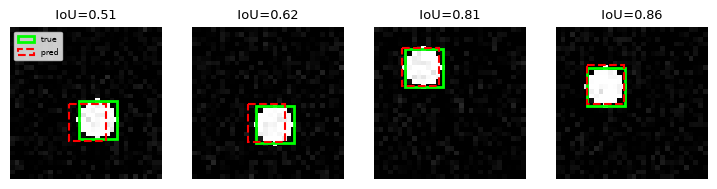
\includegraphics[width=0.85\textwidth]{figures/lesson41_fig02.png}
\caption{Predicted boxes (red, dashed) vs.\ true boxes (green) on four test scenes, with per-example IoU.}
\label{fig:l41-2}
\end{figure}

\section{Scaling this up: two families of real detectors}

This detector above only handles exactly one object per image, because a fixed-size output vector (4 numbers) can only describe one box. But real scenes have a variable, unknown number of objects. Two different families of detectors dominate the landscape:

\textbf{Two-stage (R-CNN family):} first generate a modest number of \emph{region proposals} --- candidate boxes likely to contain something, via a cheap, class-agnostic method (the original R-CNN used classical segmentation; \textbf{Faster R-CNN} (\citelink{ren2015}{Ren et al., 2015}) learns a small ``region proposal network'' instead) --- then run a classifier-plus-box-regressor (this chapter's whole architecture) on each proposal independently, exactly like running the sliding-window classifier from Chapter~\ref{ch:lesson40} but only at a handful of promising locations instead of every window. Accurate, but only as fast as (proposals) $\times$ (one forward pass) allows.

\textbf{Single-stage (YOLO, SSD):} skip proposals entirely. \textbf{YOLO} (You Only Look Once, \citelink{redmon2016}{Redmon et al., 2016}) divides the image into a coarse grid of cells, and has each grid cell directly predict (as this chapter's network does) a fixed number of boxes plus a class label plus a confidence score, all in one forward pass. \textbf{SSD} (Single Shot MultiBox Detector, \citelink{liu2016ssd}{Liu et al., 2016}) follows the same one-pass recipe but predicts boxes from \emph{several} feature-map resolutions at once (not just one final grid), so coarser layers naturally catch larger objects and finer layers catch smaller ones. To let a single cell describe objects of different aspect ratios, single-stage detectors use \textbf{anchor boxes}: several predefined box shapes (tall, wide, square) per cell, with the network predicting an \emph{offset} from each anchor rather than a box from scratch. Faster to run, historically somewhat less accurate than two-stage methods, though the gap has narrowed considerably.

Both families end with the same postprocessing step: non-maximum suppression (NMS, Chapter~\ref{ch:lesson40}) to merge the overlapping candidate boxes any real multi-object scene produces. (For simplicity, this chapter's toy detector omitted NMS by only predicting a single bounding box.)

\section{In practice: real detectors on real images}

OpenCV ships a single-stage detector, \code{cv2.FaceDetectorYN} (\textbf{YuNet}, \citelink{wu2023yunet}{Wu et al., 2023}), that follows the single-stage recipe above for faces specifically. Unlike Chapter~\ref{ch:lesson40}'s Viola-Jones cascade, it's a small single-shot CNN --- the same family as SSD above, just specialized to one class --- and it runs its own NMS internally before returning boxes. Run on the same Apollo 11 crew photo as Chapter~\ref{ch:lesson40} (Figure~\ref{fig:l41-3}), YuNet finds all three astronauts correctly, with no false positive --- an improvement over Viola-Jones's spurious detection on fabric texture. This is the payoff of a learned single-shot CNN over a cascade of hand-designed Haar-like features: richer features, trained end-to-end on real face/non-face data rather than assembled stage by stage.

\begin{figure}[h]
\centering
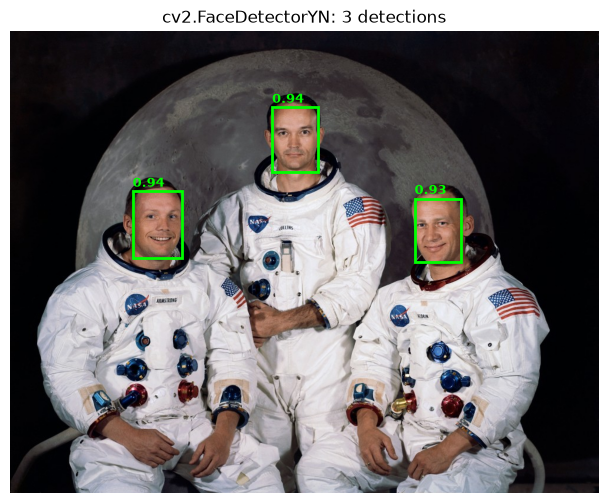
\includegraphics[width=0.75\textwidth]{figures/lesson41_fig03.png}
\caption{\code{cv2.FaceDetectorYN}: 3 detections, each with a confidence score. \attrib{Image source: NASA (public domain), via Wikimedia Commons.}}
\label{fig:l41-3}
\end{figure}

But YuNet only answers ``face or not'' --- one class. For general, multi-class detection, Faster R-CNN pretrained on \textbf{COCO} (\citelink{lin2014coco}{Lin et al., 2014}, about 330k real photos labeled across 80 object categories) is a few lines away via \code{torchvision}. This is the same ``pretrained model in one line'' pattern as Chapter~\ref{ch:lesson38}'s ResNet-18. It natively handles a variable, unknown number of objects per image --- the actual payoff of the region-proposal architecture described above.

\begin{lstlisting}
weights = torchvision.models.detection.FasterRCNN_ResNet50_FPN_Weights.COCO_V1
real_detector = torchvision.models.detection.fasterrcnn_resnet50_fpn(weights=weights)
real_detector.eval()  # frozen, no training at all -- Faster R-CNN exactly as released
\end{lstlisting}

\begin{figure}[h]
\centering
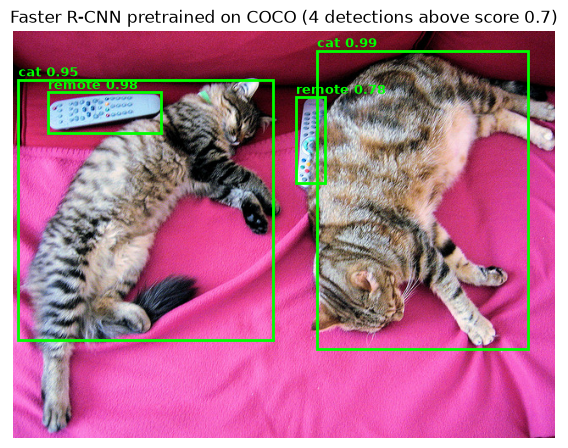
\includegraphics[width=0.7\textwidth]{figures/lesson41_fig04.png}
\caption{Faster R-CNN pretrained on COCO: 4 detections above score $0.7$. \attrib{Image source: COCO dataset (val2017, image 000000039769).}}
\label{fig:l41-4}
\end{figure}

Four confident, correct detections survive the $\text{score\_thresh}=0.7$ cutoff (Figure~\ref{fig:l41-4}) --- two cats and two remote controls, each above $0.78$ --- despite this network using only pretrained weights. Lowering the threshold reveals what the cutoff was hiding: several overlapping, lower-confidence boxes (a ``couch'' and a ``bed'' guess both covering most of the image, around score $0.54$).

\subsection*{Exercises}
\begin{enumerate}
  \item Change \code{obj\_size} in \code{make\_scene} from a fixed $8$ to a random value (e.g.\ \code{rng.integers(4, 12)}) so objects vary in size, and retrain. Does mean IoU hold up, get worse, or barely change --- and why would variable object scale be harder for a single fixed-size regression head than variable position?
  \item The loss function here is plain MSE on $(c_x,c_y,w,h)$, but the metric that matters is IoU. Replace the loss with \code{1 - iou\_batch(pred, target).mean()} (directly optimizing IoU) and compare final mean test IoU to the MSE-trained version. Real detectors (e.g.\ Faster R-CNN, YOLO variants) do exactly this with generalized IoU losses --- can you see why MSE loss and IoU metric might disagree on which of two similar predictions is ``better''?
  \item This chapter's detector has no anchor boxes and only ever handles one object. Sketch (in words) how you would modify the architecture's \emph{output} to handle up to 3 objects per image using a $3\times3$ grid where each grid cell predicts one box and a ``there's an object here'' confidence --- the core idea behind YOLO's grid.
  \item Lower \code{score\_thresh} on the real Faster R-CNN to $0.3$ and rerun. Count how many boxes appear versus at $0.7$; which of the new ones are genuinely additional objects and which are duplicates/near-misses on the cats or remotes that NMS would normally merge away?
\end{enumerate}

\vfill
\fullcode{lesson41}{lesson41_object_detection_regression}
